\documentclass[UTF8,a4paper]{ctexart}

% =========================
% 基础排版与功能宏包
% =========================
\usepackage[a4paper,margin=2.54cm]{geometry}
\usepackage{amsmath}
\usepackage{array}
\usepackage{booktabs}
\usepackage{caption}
\usepackage{float}
\usepackage{graphicx}
\usepackage{hyperref}
\usepackage{indentfirst}
\usepackage{listings}
\usepackage{longtable}
\usepackage{makecell}
\usepackage{needspace}
\usepackage{subcaption}
\usepackage{tabularx}
\usepackage{titlesec}
\usepackage{xcolor}

\hypersetup{hidelinks}
\graphicspath{{report_assets/}}

% =========================
% 字体策略：
% 1. 中文主文本由 ctex 管理；
% 2. 英文正文统一使用 Times New Roman；
% 3. 代码与等宽内容统一使用 Consolas。
% =========================
\IfFontExistsTF{Times New Roman}{
    \setmainfont{Times New Roman}
}{
    \setmainfont{Times New Roman}
}
\IfFontExistsTF{Consolas}{
    \setmonofont[Scale=MatchLowercase]{Consolas}
}{
    \setmonofont[Scale=MatchLowercase]{Courier New}
}

\setlength{\parindent}{2em}
\setlength{\parskip}{0pt}
\renewcommand{\arraystretch}{1.2}
\captionsetup{font=small,labelsep=space}
\setlength{\textfloatsep}{10pt plus 2pt minus 2pt}
\setlength{\floatsep}{8pt plus 2pt minus 2pt}
\setlength{\intextsep}{10pt plus 2pt minus 2pt}
\renewcommand{\topfraction}{0.9}
\renewcommand{\bottomfraction}{0.85}
\renewcommand{\textfraction}{0.08}
\renewcommand{\floatpagefraction}{0.8}

\titleformat{\section}{\heiti\fontsize{14pt}{21pt}\selectfont}{\thesection}{0.75em}{}
\titleformat{\subsection}{\heiti\fontsize{12pt}{18pt}\selectfont}{\thesubsection}{0.75em}{}
\titlespacing*{\section}{0pt}{1.2\baselineskip}{0.6\baselineskip}
\titlespacing*{\subsection}{0pt}{0.8\baselineskip}{0.4\baselineskip}

\definecolor{codebg}{RGB}{248,248,248}
\definecolor{codeframe}{RGB}{210,210,210}
\definecolor{codekeyword}{RGB}{0,0,160}
\definecolor{codecomment}{RGB}{0,120,0}
\definecolor{codestring}{RGB}{150,30,30}

% 代码片段样式：正文只保留少量关键实现，用于解释方法，避免替代完整源代码。
\lstdefinestyle{reportcode}{
    language=Python,
    basicstyle=\ttfamily\fontsize{10.5pt}{13pt}\selectfont,
    backgroundcolor=\color{codebg},
    frame=single,
    rulecolor=\color{codeframe},
    numbers=none,
    breaklines=true,
    showstringspaces=false,
    tabsize=4,
    keywordstyle=\color{codekeyword}\bfseries,
    commentstyle=\color{codecomment},
    stringstyle=\color{codestring}
}

\newcommand{\titlefont}{\heiti\fontsize{16pt}{24pt}\selectfont}
\newcommand{\authorfont}{\songti\fontsize{14pt}{21pt}\selectfont}
\newcommand{\affilfont}{\songti\fontsize{12pt}{18pt}\selectfont}
\newcommand{\bodyfont}{\songti\fontsize{12pt}{18pt}\selectfont}

\begin{document}
\bodyfont

\begin{center}
{\titlefont 基于 Vibe Coding 的个人主页设计与实现\par}
\vspace{1.0em}
{\authorfont Nemo Qi\par}
\vspace{0.5em}
{\affilfont （上海交通大学\quad 智能感知工程\quad enhancednemoqi@outlook.com）\par}
\end{center}
\vspace{1.0em}
{\heiti\fontsize{12pt}{18pt}\selectfont 摘要\quad}{\bodyfont 本报告记录一次使用 Codex 完成个人主页的 Vibe Coding 实践。页面以 Holo 作为技术主线，以天文观测作为视觉主线，并用 favourite movies 完成真实小数据展示。实现采用静态 HTML/CSS/JS。首屏使用横向 3D 卡片，后续内容回到纵向阅读。报告重点说明需求拆解，页面实现，截图展示和踩坑复盘。\par}
\vspace{0.5em}
{\heiti\fontsize{12pt}{18pt}\selectfont 关键词\quad}{\bodyfont Vibe Coding；个人主页；Holo；天文观测；交互设计}

\Needspace{6\baselineskip}
\section{引言}
课程作业要求使用 Vibe Coding 完成一个能体现个人特征的主页。页面需要包含自我介绍，真实小数据展示和一个可以触发的交互彩蛋，还要提交成品截图，设计说明和踩坑复盘。笔者将这个要求理解为一次小型前端作品实践：页面要能打开，内容要真实，交互要有自己的判断，最后还要能说明 AI 在哪里帮到了我，哪里需要我重新把方向拉回来。

本项目以个人 blog 作为网页形态。页面主线放在 Holo，天文观测和数理兴趣上。Holo 是公开项目，天文图像和设备照片来自个人素材，电影偏好作为真实小数据。页面只使用公开身份 Nemo Qi，保留学校，专业方向，邮箱和 GitHub 指路，头像和过于私人的内容不进入页面。成品部署在 GitHub Pages，访问地址为 \href{https://yayayayakumofloatsran.github.io/}{https://yayayayakumofloatsran.github.io/}。

\begin{figure}[H]
    \centering
    \begin{subfigure}[t]{0.48\linewidth}
        \centering
        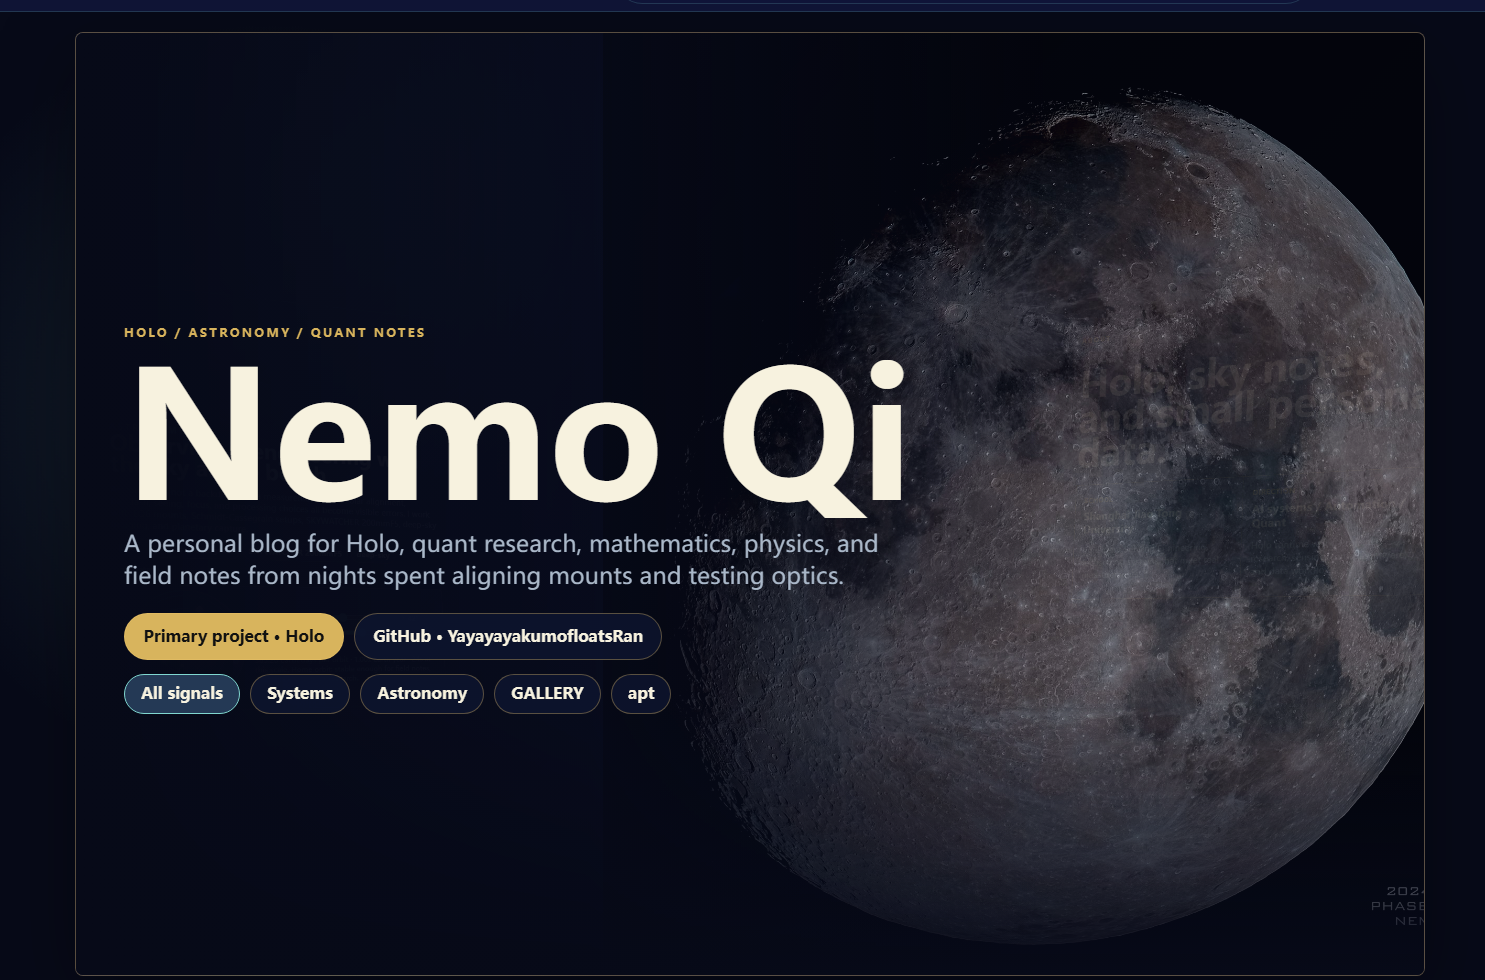
\includegraphics[width=\linewidth]{homepage-dark.png}
        \caption{默认深色首屏}
    \end{subfigure}
    \hfill
    \begin{subfigure}[t]{0.48\linewidth}
        \centering
        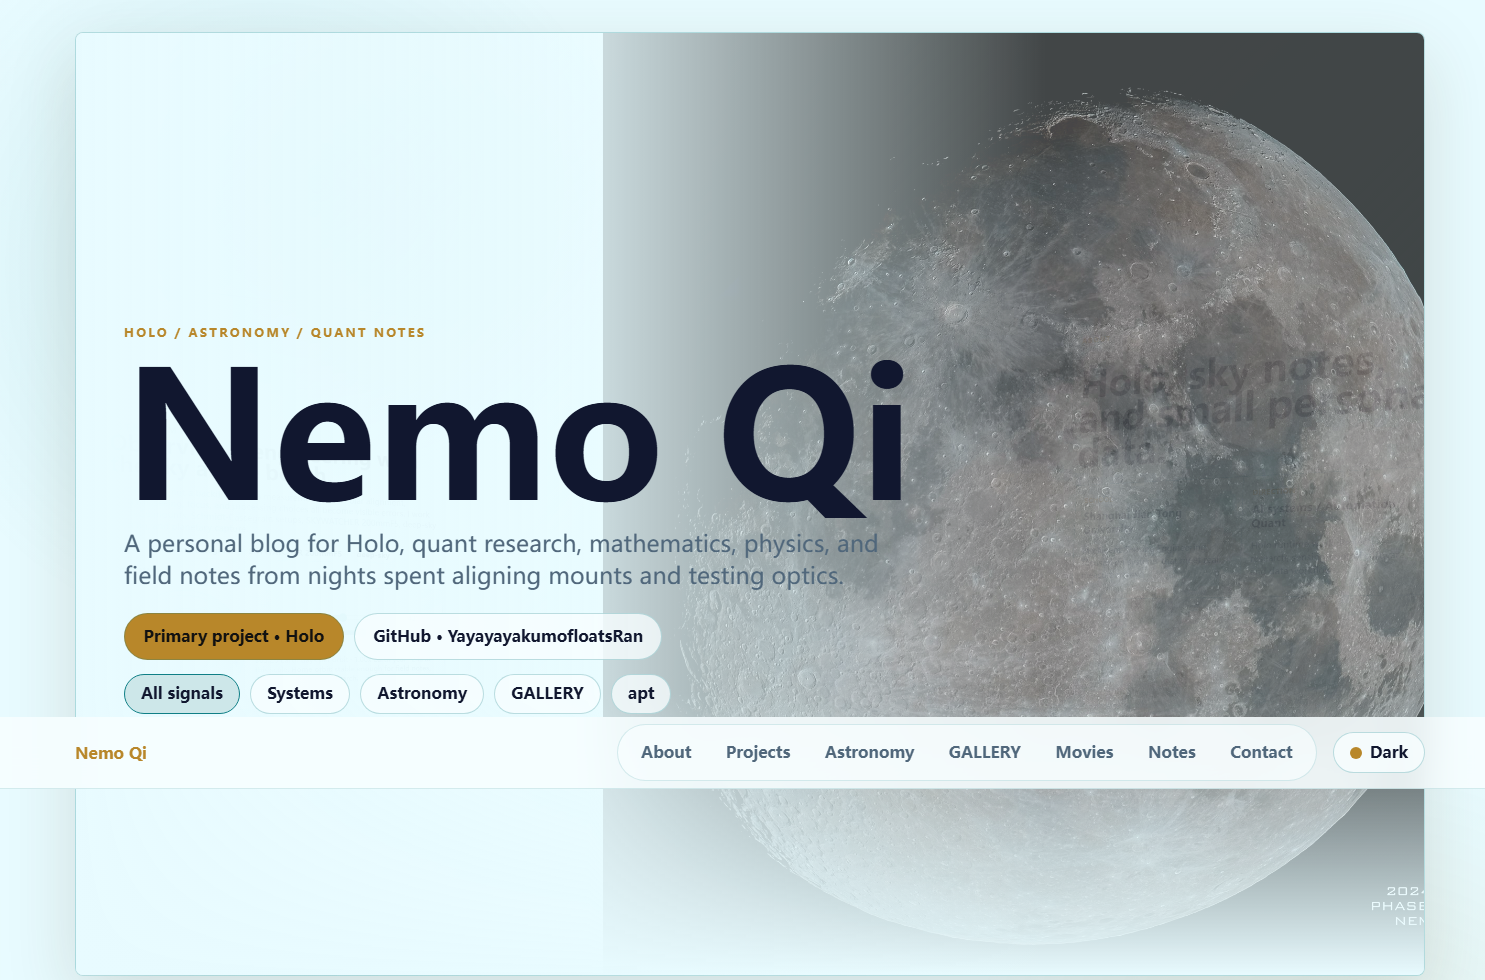
\includegraphics[width=\linewidth]{homepage-light.png}
        \caption{浅色模式对照}
    \end{subfigure}
    \caption{图 1 主页首屏主题对照。默认展示采用深色天文主题，浅色模式仅作为可切换状态保留。}
\end{figure}

\Needspace{6\baselineskip}
\section{需求拆解与设计边界}
作业说明中最关键的三个区域是自我介绍，数据可视化和交互彩蛋。我的处理方式是让 About 承担身份说明，让 Movies 承担真实小数据展示，让主题切换，横向 deck，太阳系控件，图片预览和 apt 彩蛋共同承担交互。这样安排后，页面不会停留在静态简历层面，也不会把私人信息暴露到公网。

视觉边界也在迭代中逐步收紧。用户头像被删除，月球图片中的地点信息经过公开化处理，画作中的个人签名也做了弱化。主页默认使用深色模式，深色配色以靛蓝和青色为主，金色只用于细线和重点边框。浅青色模式保留为可切换状态，报告中只展示一张对照图。


\Needspace{6\baselineskip}
\section{页面结构与视觉方案}
页面分为两段。第一段是横向 3D deck，包含 Intro，About，Projects 和 Astronomy 四张卡片。卡片使用显式边缘按钮翻页，鼠标滚轮留给纵向阅读。这个调整来自实际体验：滚轮翻页会破坏阅读节奏，也会让卡片难以停在屏幕中央。第二段从 Gallery 开始恢复传统纵向阅读，用于放置绘画素材，电影数据，Notes 和 Contact。

首屏使用月球图像作为视觉锚点。Astronomy 区展示月面，SKYWATCHER 200mm F5 牛顿反射镜，极轴镜视角和太阳系控件。Gallery 和 Movies 使用同一套图片卡片与 inspector 说明区，文字不直接压在图片上。这样能保证图片本身干净，访问者停留或点击时再获得解释。

\begin{figure}[H]
    \centering
    \begin{subfigure}[t]{0.48\linewidth}
        \centering
        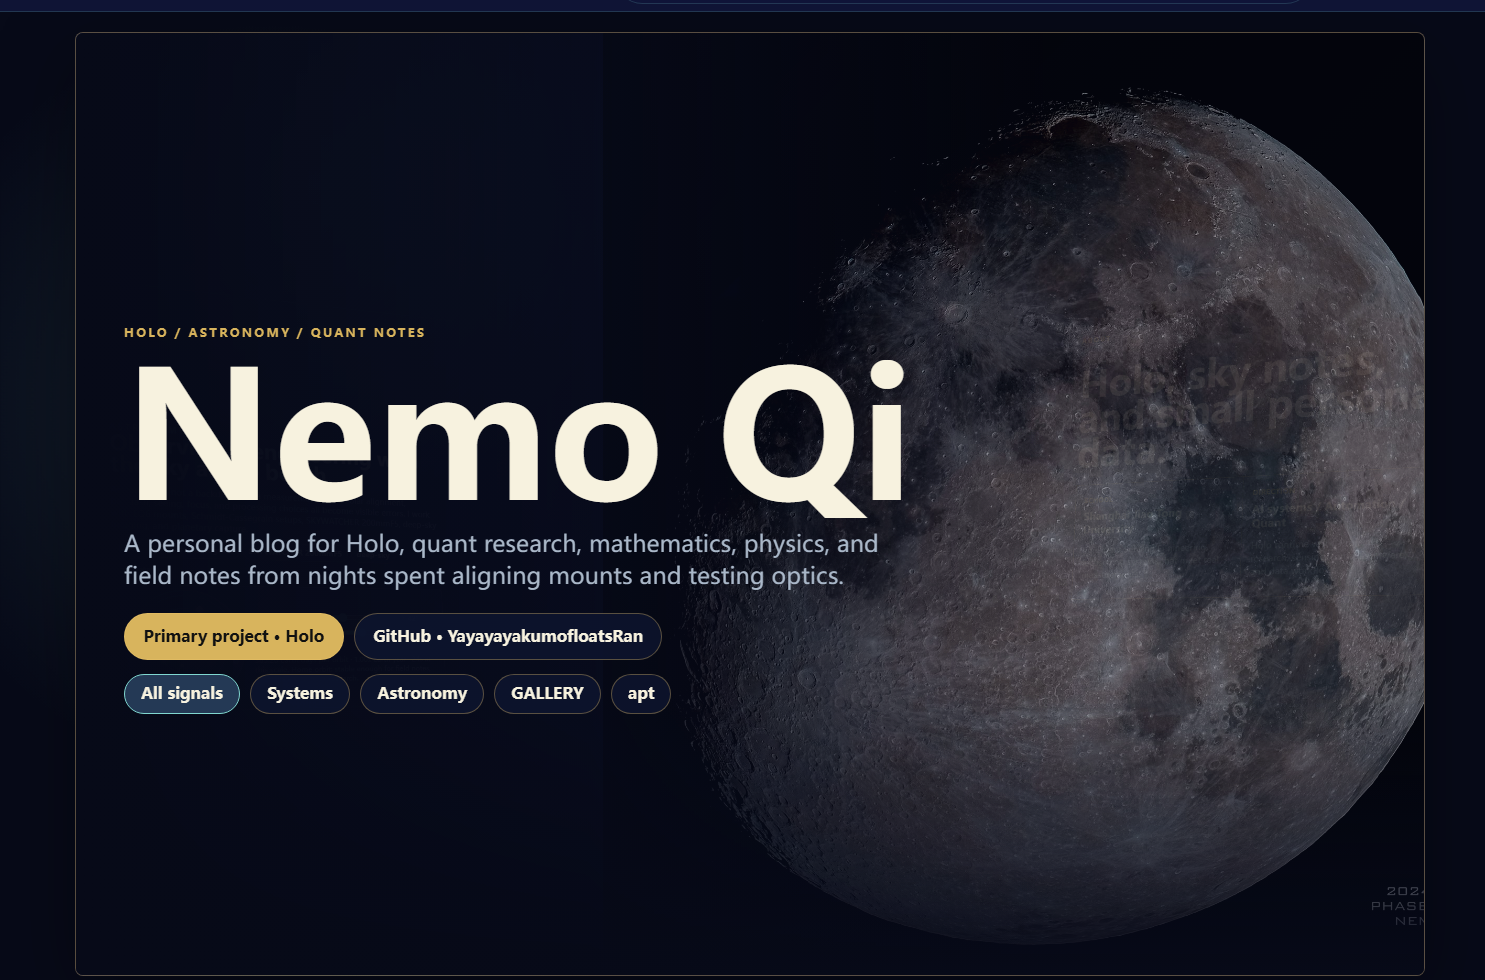
\includegraphics[width=\linewidth]{homepage-dark.png}
        \caption{Intro}
    \end{subfigure}
    \hfill
    \begin{subfigure}[t]{0.48\linewidth}
        \centering
        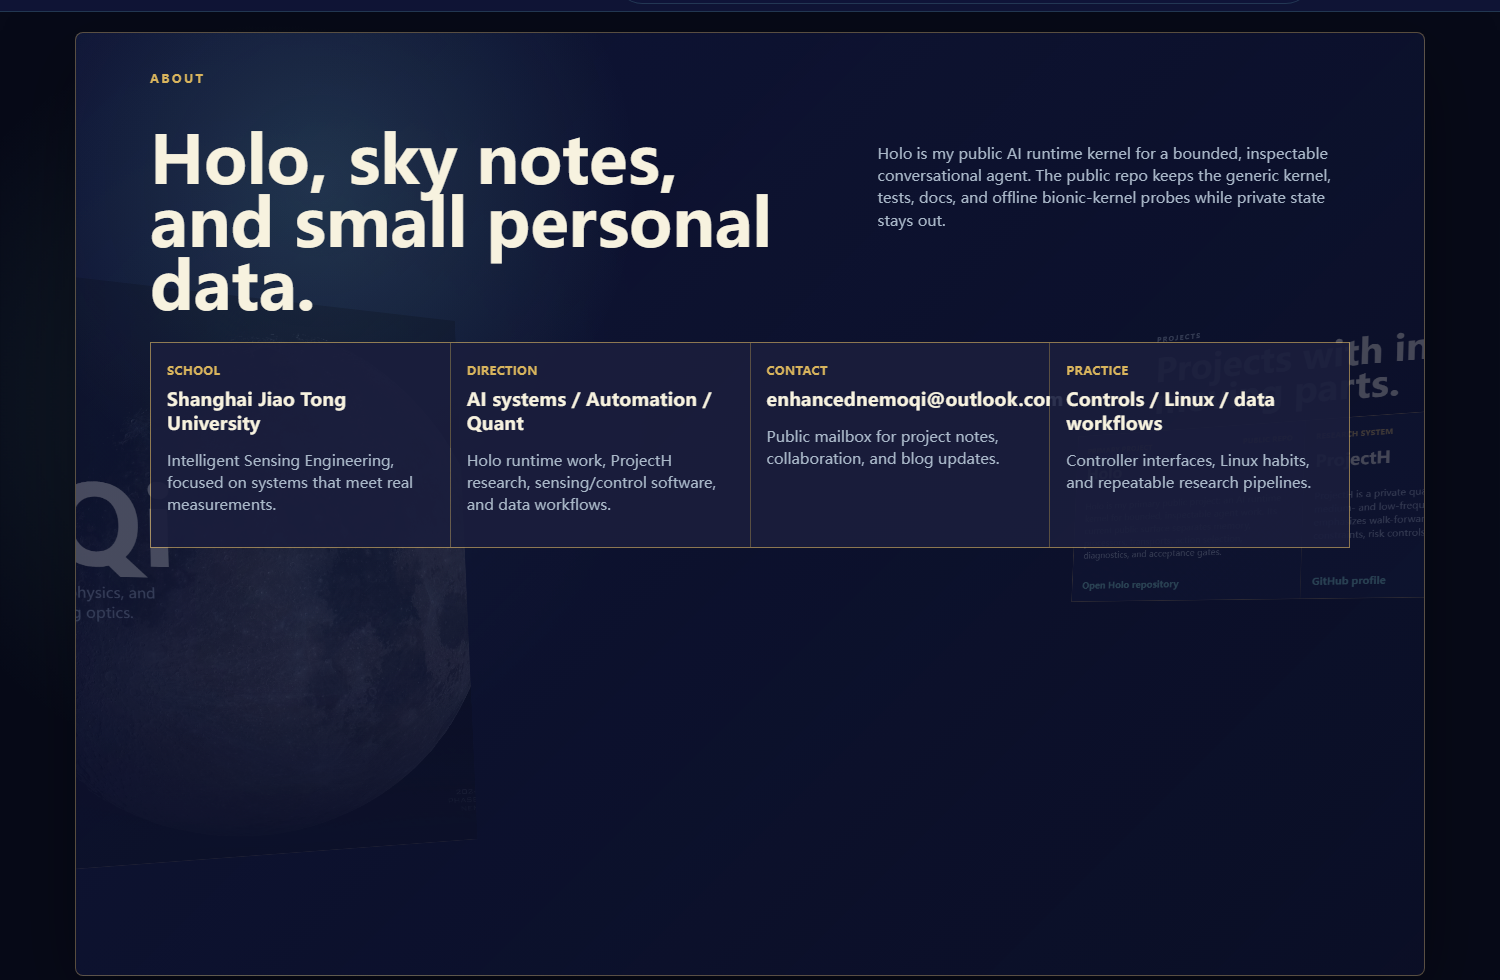
\includegraphics[width=\linewidth]{about-dark.png}
        \caption{About}
    \end{subfigure}
    \vspace{0.5em}
    \begin{subfigure}[t]{0.48\linewidth}
        \centering
        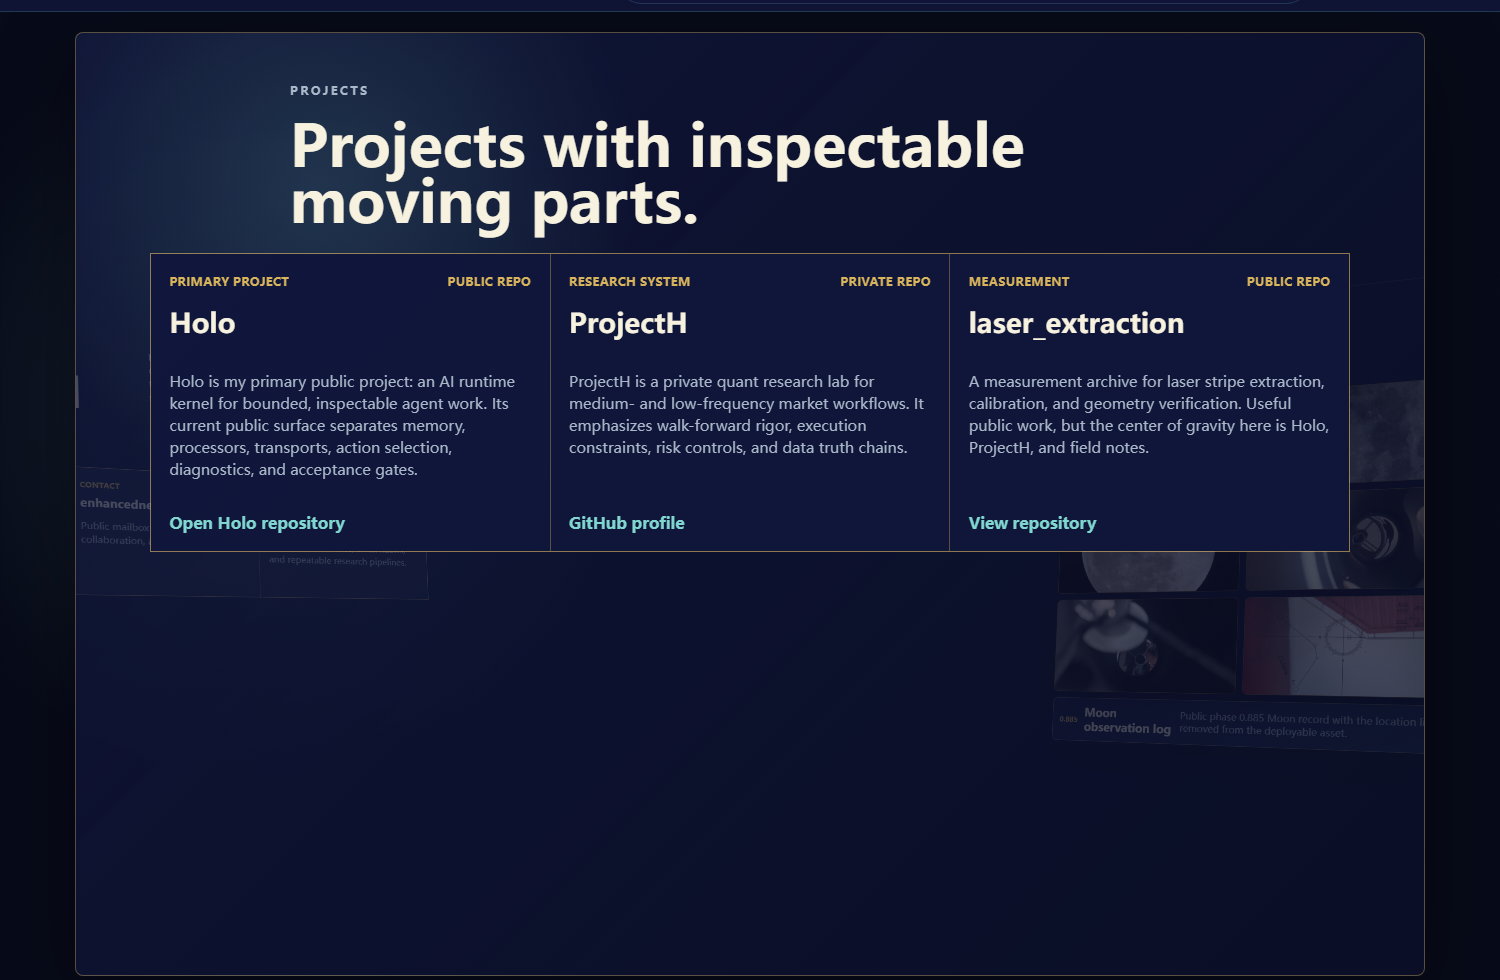
\includegraphics[width=\linewidth]{projects-dark.png}
        \caption{Projects}
    \end{subfigure}
    \hfill
    \begin{subfigure}[t]{0.48\linewidth}
        \centering
        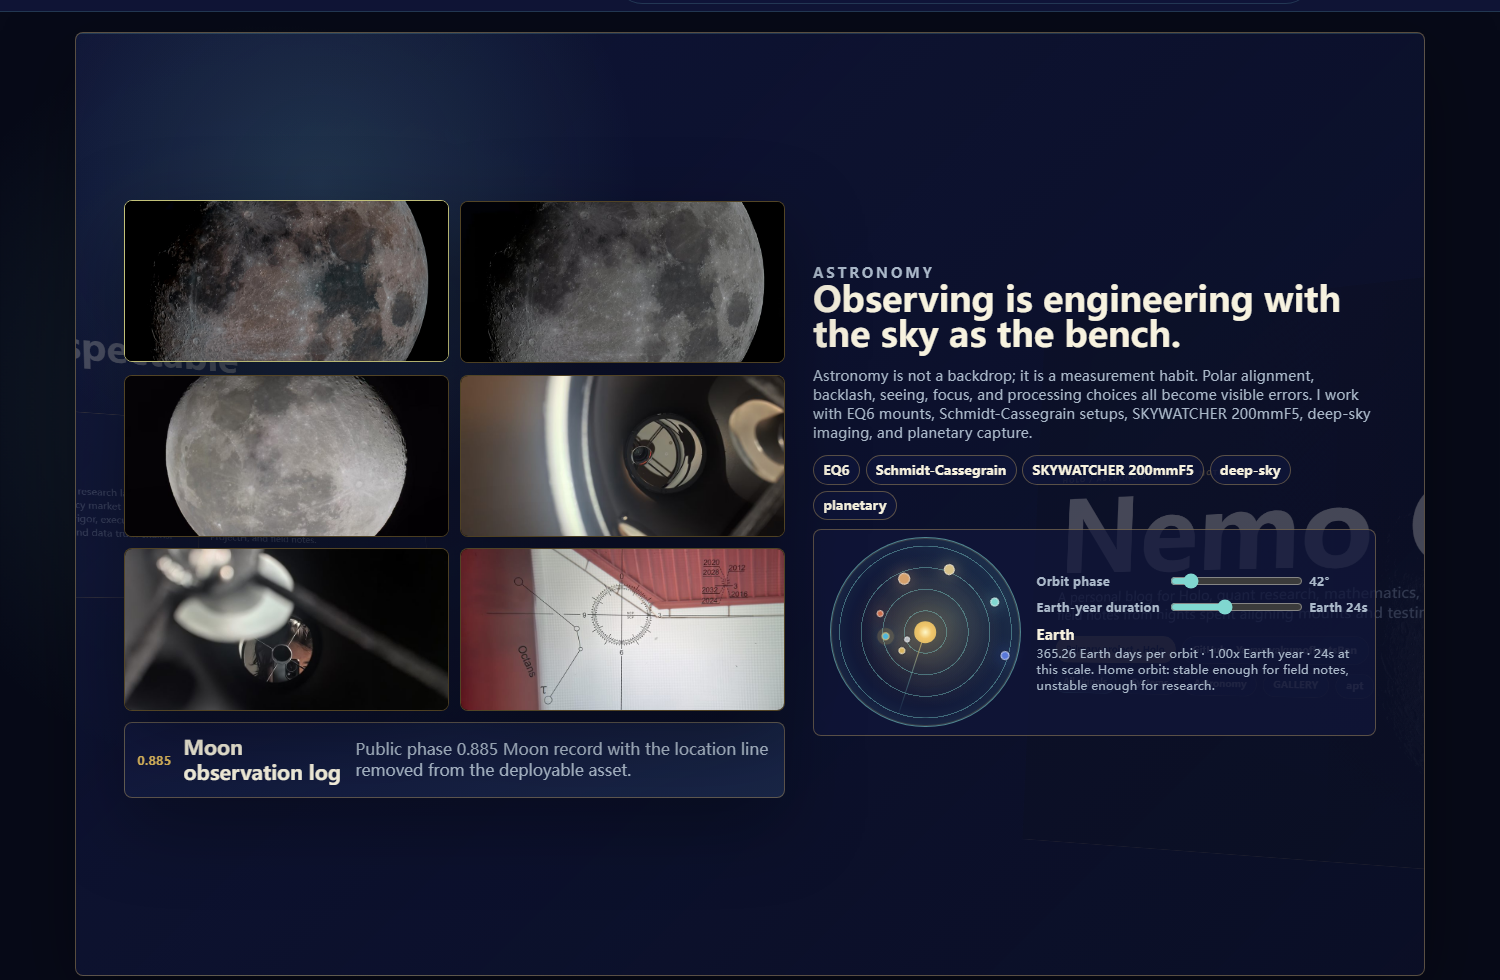
\includegraphics[width=\linewidth]{astronomy-dark.png}
        \caption{Astronomy}
    \end{subfigure}
    \caption{图 2 横向 deck 的四个主要状态。四张截图来自同一套本地渲染流程，均在深色模式下截取。}
\end{figure}

\Needspace{6\baselineskip}
\section{核心实现}
项目采用纯静态实现，核心文件是 site/index.html，site/styles.css 和 site/script.js。这种结构不依赖构建工具，便于课程提交，也便于 GitHub Pages 直接发布。部署时曾出现图片加载失败，排查后发现发布目录和资源路径不一致，随后将 site 目录作为 Pages 输出源，并保留根目录跳转文件，图片路径才稳定下来。

交互逻辑被拆成几个小模块。主题切换通过 data-theme 保存状态，横向 deck 只响应左右按钮，图片预览使用统一 lightbox，Movies 区根据电影主题统计生成条形图，Astronomy 区的太阳系控件按行星公转周期比例调整速度。这里没有追求复杂框架，重点放在可读，稳定和容易继续手工修改。

\begin{figure}[H]
    \centering
    \begin{subfigure}[t]{0.48\linewidth}
        \centering
        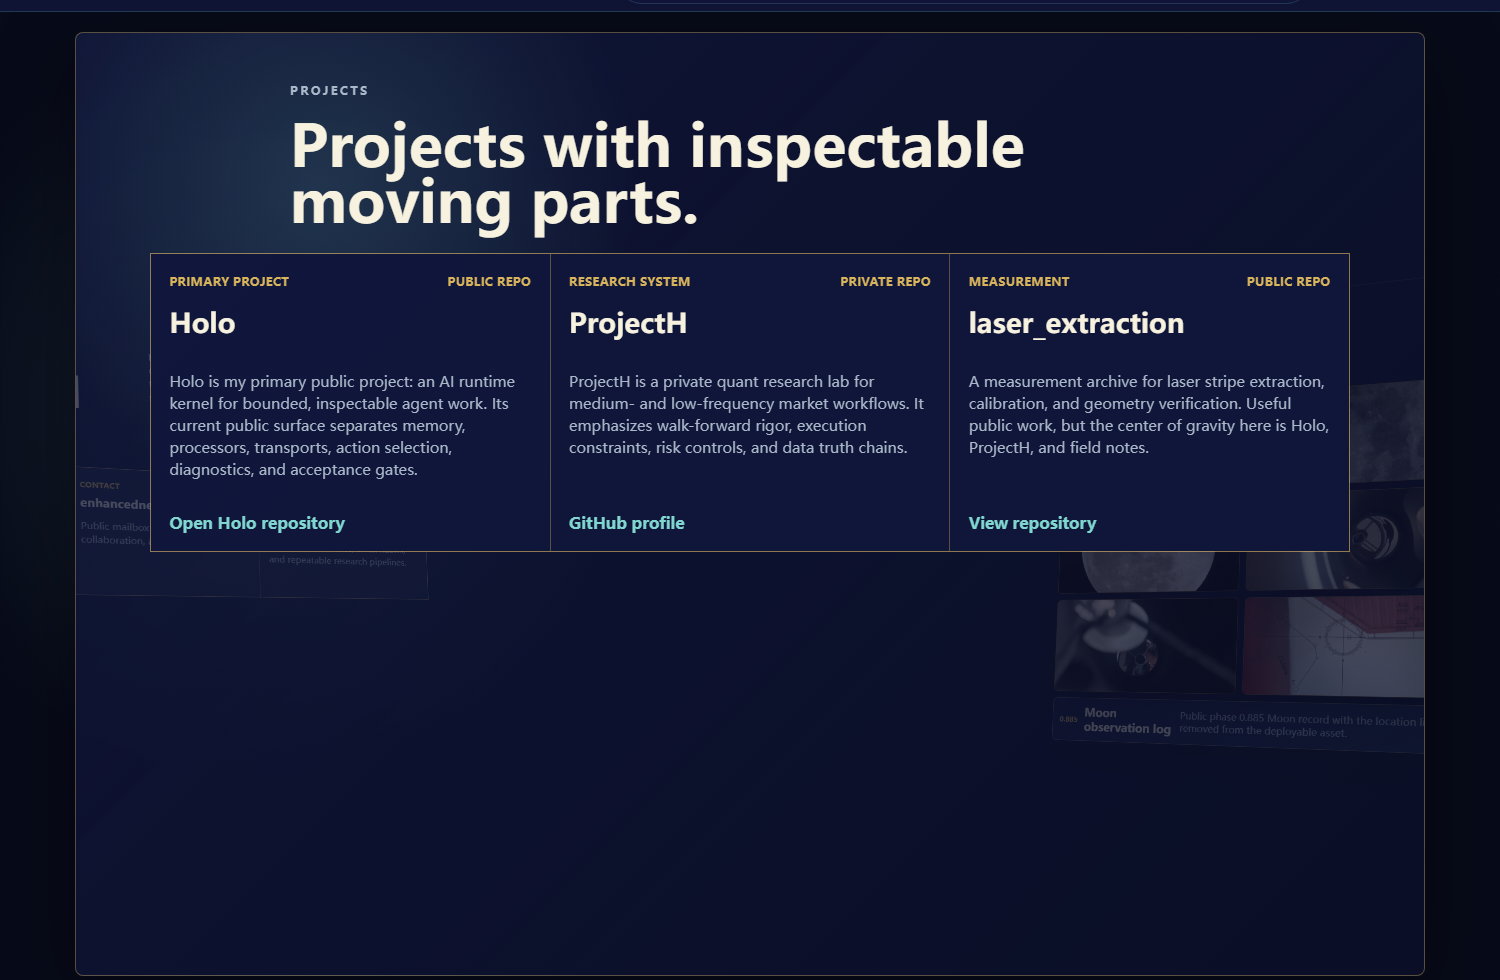
\includegraphics[width=\linewidth]{projects-dark.png}
        \caption{Projects}
    \end{subfigure}
    \hfill
    \begin{subfigure}[t]{0.48\linewidth}
        \centering
        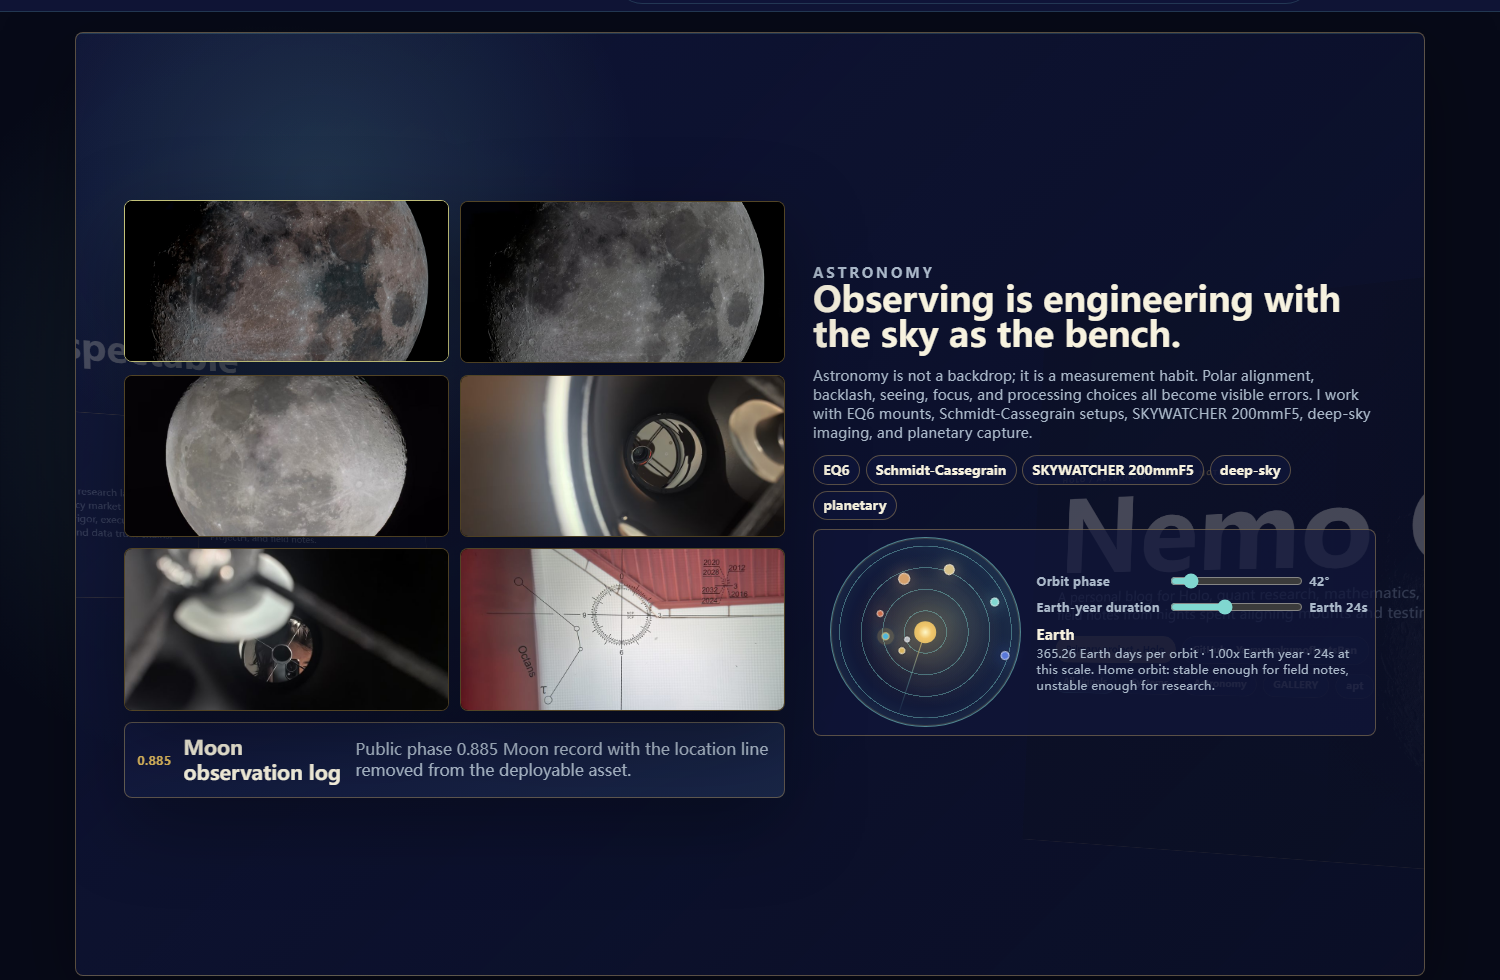
\includegraphics[width=\linewidth]{astronomy-dark.png}
        \caption{Astronomy}
    \end{subfigure}
    \caption{图 3 Projects 与 Astronomy 的并排展示。左图说明项目结构，右图展示天文观测与太阳系控件。}
\end{figure}

\Needspace{6\baselineskip}
\section{Holo 项目说明}
Holo 是我的主要公开项目。公开 README 将它定义为一个 experimental subject-runtime host，用于围绕 durable local state，replaceable processors 和 transport shells 构建 bounded, inspectable conversational agent。公开仓库只保留 generic runtime kernel，测试和文档，不包含私人 profile，长期记忆，运行数据库，传输回执和 canary artifacts。

主页中的 Holo 介绍保持简短。Projects 区只说明它是一个可检查的 AI runtime kernel，并点出 memory，processor，transport，action selection 和 acceptance gates 这些公开架构线索。README 里的 offline bionic kernel probe 已推进到 Stage35 到 Stage39，这说明 kernel v3 已经经历多轮迭代。页面因此把 Holo 放在 primary project 位置，laser\_extraction 只作为次要公开项目保留。


\Needspace{6\baselineskip}
\section{真实小数据：Favourite Movies}
作业要求一份真实属于自己的小数据。这里选用 favourite movies，因为它既真实，又能解释个人趣味。数据包括 Contact，1900，Gifted，Interstellar，The King's Speech，Batman Dark Knight，Puss in Boots 和 Ford v. Ferrari。页面没有调用外部海报接口，优先使用本地素材中已经整理好的电影图片，保证提交包离线打开时仍能显示。

可视化采用主题计数。Space 覆盖 Contact 和 Interstellar，Mind 覆盖 Gifted 和 The King's Speech，Myth 覆盖 Batman Dark Knight 和 Puss in Boots，Music 对应 1900，Velocity 对应 Ford v. Ferrari。这个结果和主页整体气质一致：一部分兴趣指向宇宙和数理，一部分兴趣指向叙事，表达和工程判断。

\begin{figure}[H]
    \centering
    \begin{subfigure}[t]{0.48\linewidth}
        \centering
        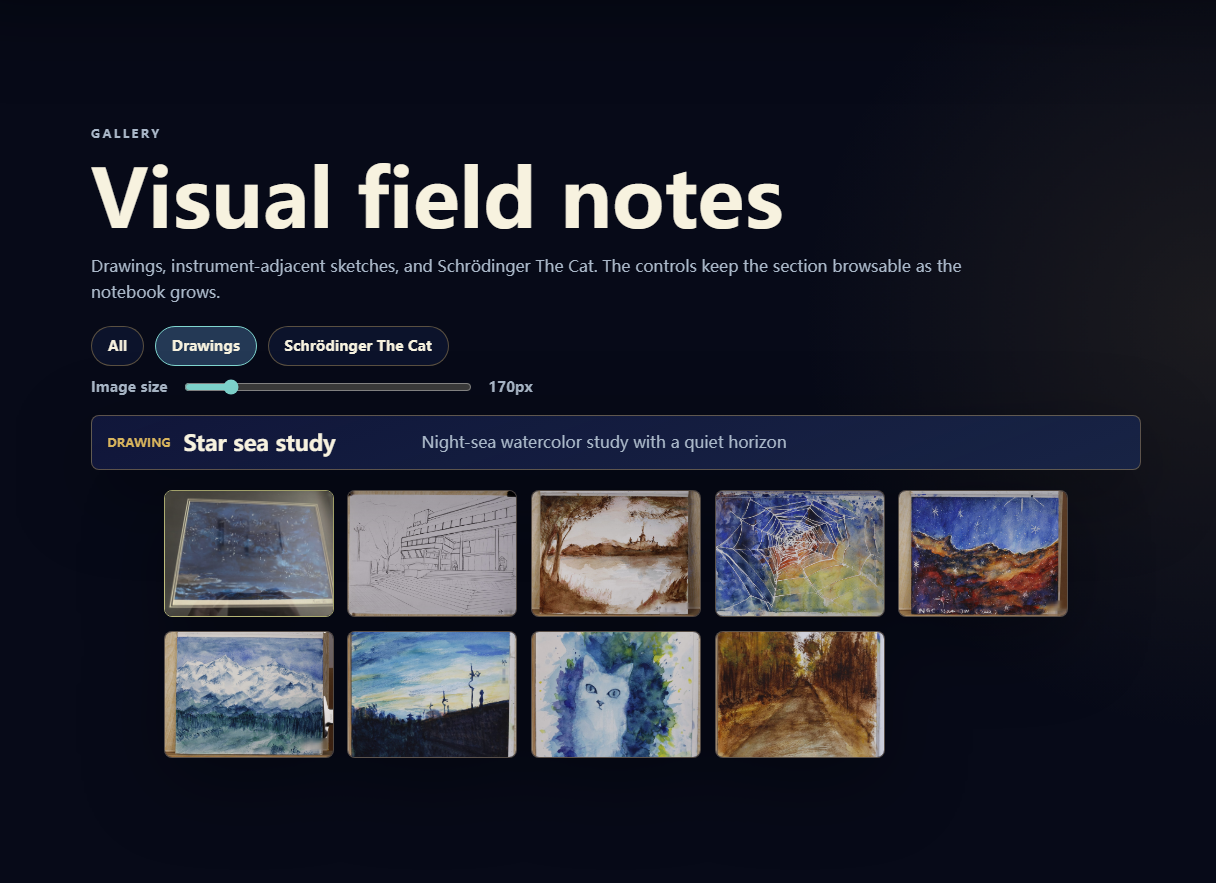
\includegraphics[width=\linewidth]{gallery-dark.png}
        \caption{Gallery}
    \end{subfigure}
    \hfill
    \begin{subfigure}[t]{0.48\linewidth}
        \centering
        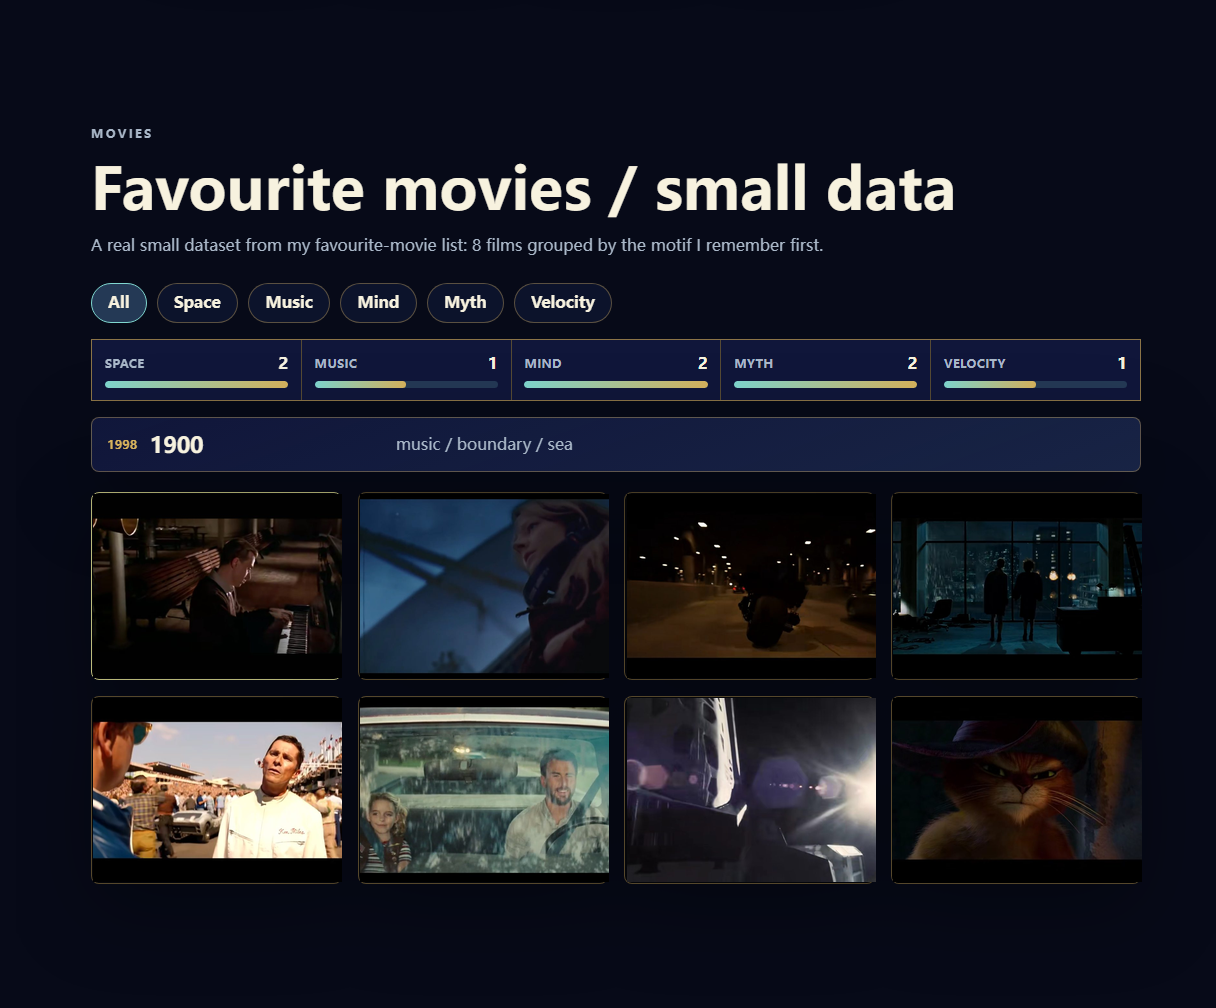
\includegraphics[width=\linewidth]{movies-dark.png}
        \caption{Movies}
    \end{subfigure}
    \caption{图 4 Gallery 与 Movies 的并排展示。绘画素材和电影小数据使用统一卡片语言，Movies 截图在八张图片完成加载后生成。}
\end{figure}
\begin{figure}[H]
    \centering
    \begin{subfigure}[t]{0.92\linewidth}
        \centering
        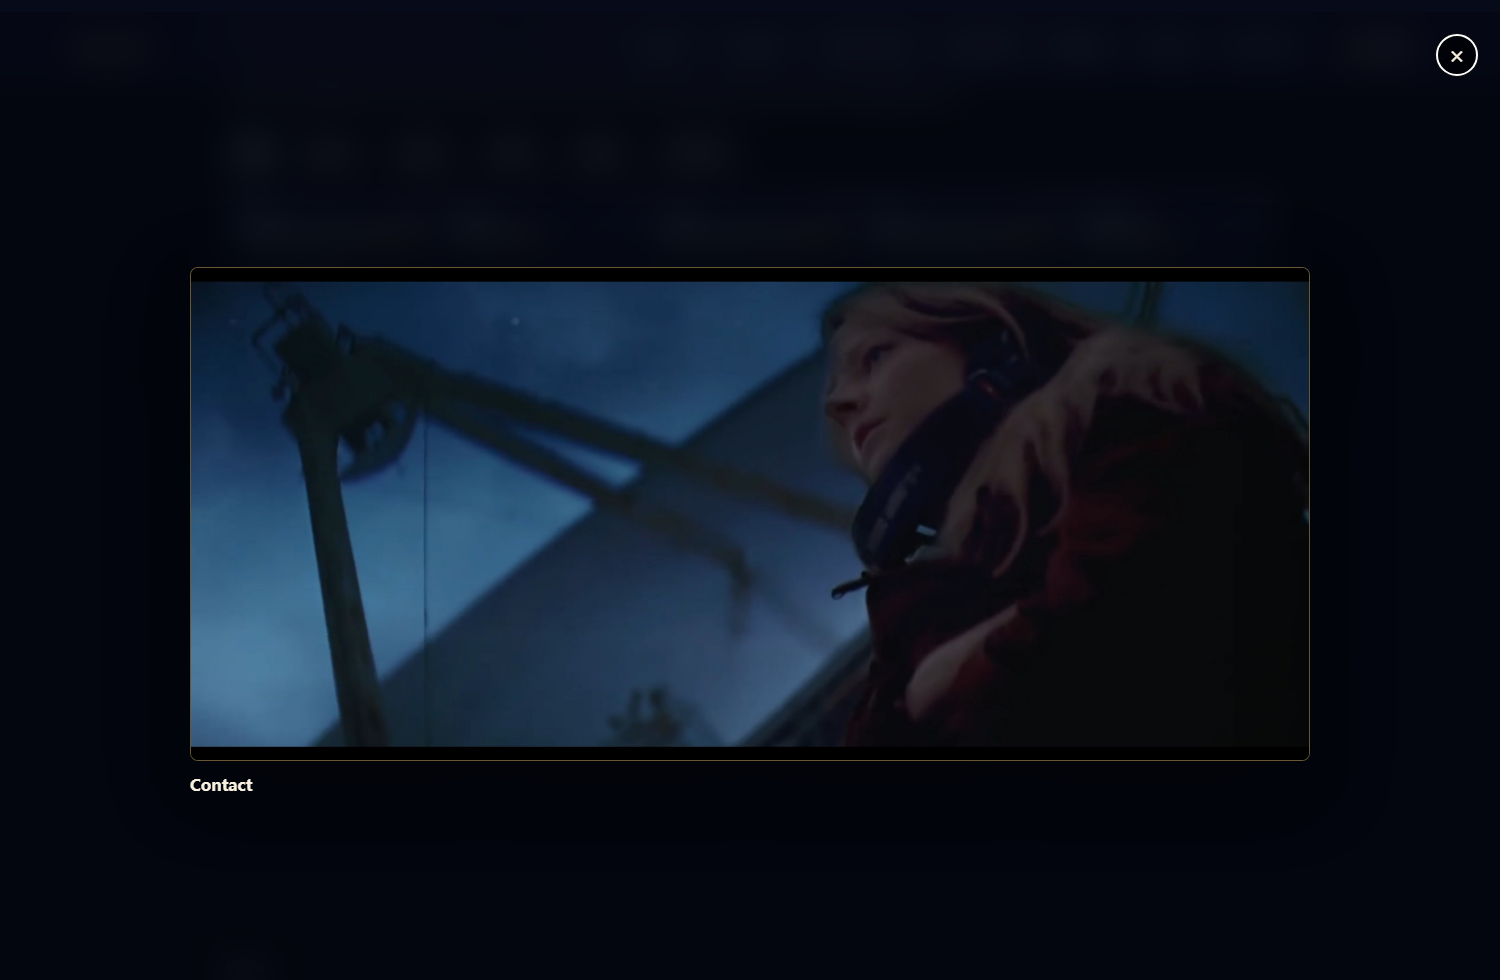
\includegraphics[width=\linewidth]{preview-dark.png}
        \caption{Image preview}
    \end{subfigure}
    \caption{图 5 图片大图预览。点击任意素材卡片后，页面以 lightbox 形式展示高分辨率图像。}
\end{figure}

\Needspace{6\baselineskip}
\section{踩坑复盘}
第一类问题是隐私边界。AI 倾向于把个人主页写得更完整，也容易保留头像占位，地点标注和签名信息。后续通过明确指令删除头像，限制公开身份，并对图片做像素处理，页面才适合放到公网。这个问题说明，公开页面的素材选择不能只看好不好看，还要检查图像里是否带有额外信息。

第二类问题是交互节奏。横向 deck 的视觉效果很好，但滚轮触发后会干扰纵向浏览。解决方法是把卡片翻页改为显式按钮，并让按钮在未触碰时近似隐形。这样保留了横向切页的立体感，也让传统阅读不受影响。

第三类问题是报告格式。AI 生成网页和 PDF 时容易走向彩色化和组件化，这与课程论文模板不一致。最后的处理方式是回到参考 TeX，逐项对齐字体，字号，行距，页边距和首行缩进。若重新开始，我会在前期就写清评分标准，公开边界，提交文件格式和报告模板，减少后期返工。


\Needspace{6\baselineskip}
\section{总结}
本次作业完成了一个可部署的个人主页。页面用 Holo 建立技术主线，用天文素材建立视觉主线，用 favourite movies 完成真实小数据展示，并用主题切换，横向 deck，太阳系控件，图片预览和 apt 彩蛋补足交互。

这次实践也让我更清楚地看到 Vibe Coding 的分工。AI 适合快速搭建结构，补齐样式和实现交互；人的工作是不断收紧边界，判断审美，检查隐私，并把作品重新拉回作业要求。最终版本仍然保留可继续手工修改的空间，后续可以把 Notes 扩展成真正的 blog 内容。


\end{document}
